%------------------------------------------------------------------------
% Template file for the submission of papers to IUCr journals in LaTeX2e
% using the iucr document class
% Copyright 1999-2013 International Union of Crystallography
% Version 1.6 (28 March 2013)
%-----------------------------------------------------------------

\documentclass[preprint]{iucr}              % DO NOT DELETE THIS LINE
\usepackage{verbatim}
\usepackage{amsmath}
\usepackage{algorithm, algpseudocode}
\usepackage[latin1]{inputenc}
\usepackage{graphicx}
\usepackage{amssymb}
\usepackage{color}
\usepackage{comment}
\usepackage{tikz}
\usetikzlibrary{shapes.geometric, arrows}
\usepackage{lscape}
\usepackage{array}

\begin{comment}
\algnewcommand\algorithmicinput{\textbf{Input:}}
\algnewcommand\INPUT{\item[\algorithmicinput]}
\algnewcommand\algorithmicoutput{\textbf{Output:}}
\algnewcommand\OUTPUT{\item[\algorithmicoutput]}
\end{comment}

\newcommand\memonazar[1]{{\color{red}{\MakeUppercase{Nazar's comment: #1}}}}
%\newcommand\memonazar{}
\newcommand\memosaadia[1]{{\color{blue}{Saadia's comment: #1}}}
% \newcommand\memocorrection[1]{{\color{blue}{Edited : #1}}}
% \newcommand\memosaadia{}

\newcommand\dsr{Debye-Scherrer ring}
\newcommand\dsrs{Debye-Scherrer rings}

\newcommand{\norm}[1]{\left\lVert #1 \right\rVert}

     %-------------------------------------------------------------------------
     % Information about journal to which submitted
     %-------------------------------------------------------------------------
     \journalcode{J}              % Indicate the journal to which submitted
                                  %   A - Acta Crystallographica Section A
                                  %   B - Acta Crystallographica Section B
                                  %   C - Acta Crystallographica Section C
                                  %   D - Acta Crystallographica Section D
                                  %   E - Acta Crystallographica Section E
                                  %   F - Acta Crystallographica Section F
                                  %   J - Journal of Applied Crystallography
                                  %   M - IUCrJ
                                  %   S - Journal of Synchrotron Radiation

\begin{document}                  % DO NOT DELETE THIS LINE

     %-------------------------------------------------------------------------
     % The introductory (header) part of the paper
     %-------------------------------------------------------------------------

     % The title of the paper. Use \shorttitle to indicate an abbreviated title
     % for use in running heads (you will need to uncomment it).

\title{Automatic Debye-Scherrer Elliptical Ring Extraction via a Computer Vision Approach}
%\shorttitle{Short Title}

     % Authors' names and addresses. Use \cauthor for the main (contact) author.
     % Use \author for all other authors. Use \aff for authors' affiliations.
     % Use lower-case letters in square brackets to link authors to their
     % affiliations; if there is only one affiliation address, remove the [a].

\author[a]{Saadia}{Shahzad}%{saadia.shahzad@pucit.edu.pk}
\author[a]{Nazar}{Khan}%{nazarkhan@pucit.edu.pk}
\author[a]{Zubair}{Nawaz}%{znawaz@pucit.edu.pk}
\author[b]{Claudio}{Ferrero}%{claudio.ferrero@esrf.fr}
\author[b]{J\'er\^ome}{Kieffer}%{jerome.kieffer@esrf.fr}

\aff[a]{PUCIT, Allama Iqbal Campus, University of the Punjab, Lahore,  
\country{Pakistan}}
\aff[b]{The European Synchrotron, 71 avenue des Martyrs, 38000 Grenoble
\country{France}}

     % Use \shortauthor to indicate an abbreviated author list for use in
     % running heads (you will need to uncomment it).

%\shortauthor{Soape, Author and Doe}

     % Use \vita if required to give biographical details (for authors of
     % invited review papers only). Uncomment it.

%\vita{Author's biography}

     % Keywords (required for Journal of Synchrotron Radiation only)
     % Use the \keyword macro for each word or phrase, e.g. 
     % \keyword{X-ray diffraction}\keyword{muscle}

%\keyword{keyword}

     % PDB and NDB reference codes for structures referenced in the article and
     % deposited with the Protein Data Bank and Nucleic Acids Database (Acta
     % Crystallographica Section D). Repeat for each separate structure e.g
     % \PDBref[dethiobiotin synthetase]{1byi} \NDBref[d(G$_4$CGC$_4$)]{ad0002}

%\PDBref[optional name]{refcode}
%\NDBref[optional name]{refcode}

\maketitle                        % DO NOT DELETE THIS LINE

\begin{abstract}
The accurate calibration of powder diffraction data acquired from area detectors
using calibration standards is a crucial step in the data reduction process to
attain high-quality one-dimensional patterns.  
% The precise determination of peak positions and intensities of a sample is
% required for any quantitative analysis, like e.g. the Rietveld refinement. 
A novel algorithm was developed for extracting Debye-Scherrer rings
automatically by using an approach based 
%on well known \memosaadia{(Dr. Nazar
%says "well known" should be replaced by some synonym of "novel". As we have
%developed a new technique in CV, its not trivial in CV)} 
on computer vision and pattern recognition techniques.    
The presented technique requires no human intervention and, unlike previous
approaches, makes no restrictive assumptions on the diffraction setup and/or
rings.  
It can detect complete rings as well as portions of them, and works on several
types of diffraction images with various degrees of ring graininess and detector
non-orthogonality with respect to the incoming beam.  

\end{abstract}


     %-------------------------------------------------------------------------
     % The main body of the paper
     %-------------------------------------------------------------------------
     % Now enter the text of the document in multiple \section's, \subsection's
     % and \subsubsection's as required.

\section{Introduction}

The increasingly wider use of area detectors for X-ray powder diffraction (XRPD)
measurements at advanced synchrotron light sources has witnessed an outstanding
success and paved new avenues to numerous bleeding-edge experiments exploiting
nanosized X-ray beams \cite {dinnebier2012future}.   
The enormous gains of 2-D data collections are the very short exposure times
(down to some microseconds), the excellent data statistics and, last but not
least, the extremely reduced duration of an experiment, as compared to just a
very few years ago. Nowadays, in the frame of an XRPD mapping experiment one may
collect as many as over 125,000 good quality frames in less than three hours by
using e.g. an Eiger detector [\cite{johnson2012capturing} ,
\cite{gorfman2014sub}].      

Although in most measurements the detector is placed orthogonal and central to
the incoming beam cone that geometrically intercepts the detector plane along
circles (Debye-Scherrer rings), in the most general case the detector is tilted
and offset with respect to the primary beam axis. 
In this case the
Debye-Scherrer rings can take the form of any conical section (ellipse,
hyperbola and parabola or even pairs of straight lines).     
In the vast majority of cases the powder patterns are actually ellipses. The
customary practice is to azimuthally integrate the image along the ellipses
\cite{hammersley1996two}, thus reducing the amount of information by the square
root of the number of pixels and consequently the disk space \cite
{dinnebier2012future}.    

Since the experimental setup for powder diffraction measurement has been
extensively described elsewhere (see e.g. the review in
\cite{lavina2014modern}), we will focus essentially on the calibration
procedure. To this effect, one needs to determine and refine numerically the
experimental parameters of the beam centre, the sample-to-detector distance, in
some particular cases the X-ray wavelength and the spatial orientation of the
detector with respect to the beam \cite{de2014xrdua}. 
Typically, high quality patterns of standard samples are used to determine and
refine the required parameters.  
Several methods have been used for refining the calibration parameters [see e.g.
\cite{dinnebier2012future} and references therein, \cite{de2014xrdua},
\cite{tantau2014high}, \cite{lutterotti2014rietveld}].  
The calibration process was totally manual for early experiments. 
Some semi-manual approaches were developed afterwards; which estimate parameters 
on manually marked rings.

Well-known computer programs commonly employed for calibration purposes and for 
analysing diffraction images include Fit2d \cite{hammersley2016fit2d}, Two2One
\cite{vogel2005two2one}, Powder3d \cite{hinrichsen2006powder3d}, Datasqueeze
\cite{heiney2005software} and PyFAI \cite{kieffer2013pyfai}. 

Pattern recognition techniques were developed to estimate calibration parameters
featuring high accuracy along with a large degree of automation
[\cite{rajiv2007automatic}, \cite{cervellino2006folding}].  
However, these approaches make restrictive assumptions about the diffraction
setup and/or the diffraction rings. 

Several synchrotron sources are currently following update programs to face the
new challenges posed by science and technology.  
% The instrumentation is also being upgraded, driven by the needs of the beamlines, 
% and notably in X-ray mirror engineering, diamond technologies, nano-focussing 
% optics, pixel detectors, on-line data analysis and high-rate data collections. 
The size of the beam is becoming of the same order of magnitude of the grains in
the powder used. 
In this case, the problem tends to become that of diffraction from single
crystals, with less random orientations of the crystals. 
The diffraction pattern shows more scattered peaks than well-defined rings. 
As it is very hard to reduce even further the size of grains in the powder,
partly due to issues related to nanoscopic powder hazard, one has to deal with
this problem at the image processing level.  

The basic task of the present work has been to develop a novel algorithm for
extracting diffraction rings, which should not need human intervention to
capture the rings or portions of them.  
Another point is that it should work on several types of images, with various
degrees of graininess. 
The basic idea is to use a computer vision approach to automatically analyse the
two-dimensional diffraction frames and search and classify the ring-like shapes
by sub-families of conic sections, the geometric parameters of which would
enable the refinement of the instrumental parameters.   

In the following sections the different steps toward the automatic extraction of
the Debye-Scherrer rings are illustrated, starting from the image
pre-processing, followed by morphological dilation and thinning operations
(section \ref{sec:gapFilling}).   
These morphological operations are parts of an algorithm to control the growth
of regions bearing conic candidates (section \ref{regGrow}) and use an
incremental detection mechanism (section \ref{subsec:EllipseGrow}).  
The algorithm has been validated for ellipses. 
The main features of the ellipse harvesting strategy are then explained
introducing suitable convergence and ranking criteria (section
\ref{sec:ellipseEval}) and then improving detection using family constraint for
ellipses (section \ref{sec:family}).   
Finally, a comparison between the suggested method and existing ring detection
schemes is discussed (section \ref{sec:compr}). 


\section{Computer-vision aided ring extraction}
As mentioned in the introduction, {\dsrs} fitting is the core of XRPD data
calibration. 
We propose a computer-vision-aided algorithm to automatically extract {\dsrs} in
XRPD images. 
The detection of these rings allows the calibration of the experiment
\cite{pyFAI_2015}. 
The calibration process is based on obtaining actual elliptic rings
individually. 
Manual marking on the rings can be slow as well as error prone. 
Our algorithm can be used to automate this process.


\begin{figure}
\centering

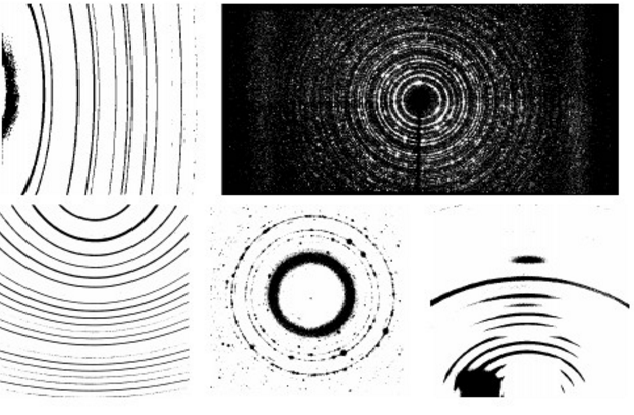
\includegraphics[width=.85\linewidth]{Figures/dsrs_example.png}

\label{fig:examples}
\caption{Examples of \dsrs{} images acquired on various synchrotron beamlines.}
\end{figure}

As shown in Figure \ref{fig:examples}, segments of Debye-Scherrer rings can
appear in a wide variety of ways from almost circular to elliptical, parabolic
and even almost linear. 
The modular structure of certain detectors (i.e. Pilatus detectors from Dectris) 
may produce ring which do not appear to be contiguous.   
% In addition, the detection apparatus can lead to both regular and irregular
% artifacts.
This makes the automatic detection of such rings or ring portions a challenging
task. 

Considerable research exists on the ellipse fitting problem when points
representing an ellipse are provided \textit{a priori}
\cite{gander1996least,fitzgibbon1999direct,kanatani2008compact}. However, the
problem of grouping points that represent elliptical regions has received less
attention (e.g. 
\cite{qiao2007arc,chia2011split,wong2012survey,puatruaucean12A}).     

If there are multiple ellipses in one image, it is hard to identify which set of
points lie on which ellipse. 
This could be done by viewing the image and marking points manually but it is
tedious and very time consuming to identify all points of one ellipse from a
list of all points in the image.  
As demonstrated in the Figure \ref{fig:chickenandegg}, if we can identify the
points lying on one ellipse, ellipse fitting is trivial. 
On the other hand, if we know the parameters of an ellipse, obtaining the points
that lie on ellipse is trivial. 
However, in the absence of both (points as well as ellipse), ellipse detection
is a challenging task and can be treated as a latent variable problem. 

\begin{figure}
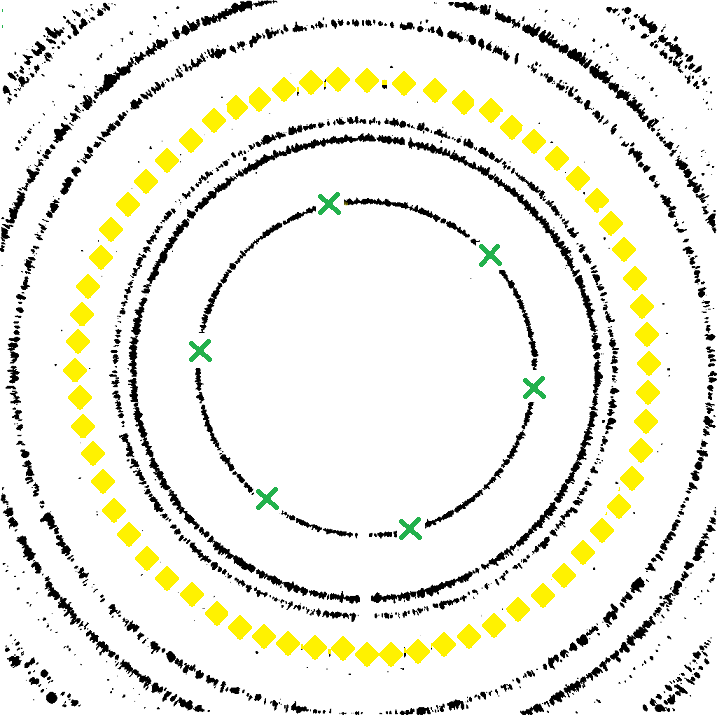
\includegraphics[width=.45\linewidth]{Figures/max1_points_on_ellipse_new.png}
\label{fig:chickenandegg}
\caption{Above image is representing a diffraction pattern. 
Upon identifying some points of a candidate ellipse (green crosses), an ellipse
can be fitted through these points. 
Conversely, knowing the ellipse parameters all points on/near that ellipse can
be identified (yellow diamonds)}
\end{figure}

We approached this problem in an incremental fashion, similar in spirit to the
incremental nature of the expectation maximisation (EM) algorithm
\cite{dempster1977maximum} used for solving latent variable problems.  
Accordingly, we name our algorithm as incremental ellipse detection (IED).

We start with an initial region (set of points) and fit an ellipse to it.
Then, we select additional points that lie close to both, the region and the
corresponding fitting ellipse and add these to the region. 
A new fitting ellipse is then adjusted to this expanded region and the process
is repeated until no more points can be added to the region. 
Other regions in the image can similarly be processed in sequence to obtain all
elliptical region estimates i.e. the {\dsrs}. 

After initial pre\-processing (section \ref{sec:gapFilling}), we merge sets of
points to identify potential regions (section \ref{regGrow}), then we detect
ellipses using the IED algorithm (section \ref{subsec:EllipseGrow}).  
The details of the algorithm and its sub-procedures are presented in the
following subsections Pseudo-code of our IED algorithm is presented in Appendix
A.  

\subsection{Gap Filling} \label{sec:gapFilling}
By inspecting the \dsrs{} in an image, we can find out that they can be
comprised of unconnected sets of pixels (see Figure \ref{fig:examples}). 
There can be gaps along the rings.
We pre-process the data to fill these gaps.
This gap-filling enables to find connected elliptic arcs more accurately.

Let $I$ denotes an image having {\dsrs}.
Since the range of pixel intensities in such images can vary significantly, we
force the intensities to lie between 0 and 255 via an affine rescaling as
follows:  

\begin{align} \label{eq:affine}    
    I_{x,y} = \frac{I_{x,y} - \min(I)}{\max(I) - \min(I)} * 255    
\end{align}

We smooth the image $I$ with rotationally symmetric Gaussian lowpass filter of
size 2x2 with one(1) standard deviation. 
After that derivatives in $x$ and $y$ directions are computed using Equation
(\ref{eq:gradX}) and Equation (\ref{eq:gradY}). 

\begin{figure}
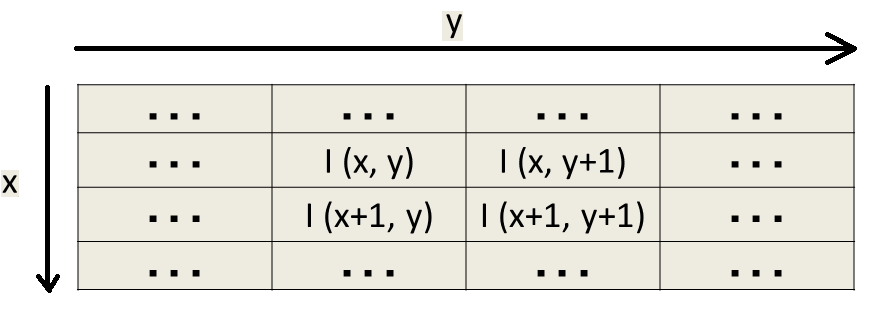
\includegraphics[width=.45\linewidth]{Figures/Gradiant_Pixels_grid.png}
\label{fig:grid}
\caption{For the pixel $I(x,y)$, we use its neighbouring pixels to compute the
derivatives in $x$ and $y$ directions.} 
\end{figure}


\begin{align} \label{eq:gradX}
I_{x}(x,y) = \frac{(I(x+1,y)-I(x,y)) + (I(x+1,y+1)-(I(x,y+1))}{2}
\end{align}

\begin{align} \label{eq:gradY}
I_{y}(x,y) = \frac{(I(x,y+1)-I(x,y)) + (I(x+1,y+1)-(I(x+1,y))}{2}
\end{align}

The gradient magnitude, $m(x,y)$, is the square root of the sum of the squares
of these two derivatives, as shown in Equation (\ref{eq:gradMag}). 
\begin{align} \label{eq:gradMag}
m(x,y)&=\sqrt{(I_{x}(x,y))^2+(I_{y}(x,y))^2}
\end{align}

Then, we select pixels whose gradient magnitudes are greater than or equal to
the 90th percentile of all gradient magnitudes, producing a binary image. 

The connectivity among pixels along the rings can be improved through a simple
morphological operation of dilation. 
 We dilate our image by using the structuring element of size 3x3 containing all
 ones. 
While dilation can fill gaps between pixels, it can also lead to unnecessarily
thicker boundaries. 
Therefore, dilation is followed by a thinning procedure to neutralise the
thickening effect of dilation while retaining its gap-filling effect. 

Gap filling enhances the image quality and makes the image more suitable for
harvesting connected regions in the region-growing procedure (section
\ref{regGrow}).  
Subsequent region growing steps produce much better results when gaps are
processed by this dilation and thinning sequence. 
This procedure leads eventually to more accurate and faster ellipse detection. 

Figure \ref{fig:Dilt_Thin} demonstrates the effect of dilation and thinning.
One can see that original images have gaps along the rings (first column).
The first row shows full images, the second shows a zoomed-in portion of one
ellipse from the image, the third row displays the same zoomed-in portion after
region growing and the fourth row shows the full image after region growing.  
The second column shows the effect of dilation for both the full and zoomed-in
images. 
It can be observed that dilation fills gaps and also thickens the boundary,
while thinning retains the filling as shown in the third column for both the
zoomed-in and the full image.  
It can also be observed that the process of dilation and thinning yields a
result that is closer to the original regions (fourth row) but more suitable for
finding connected regions.  
Each colour represents a different region.

In all subsequent figures (including figures in section \ref{sec:compr}, the
{\dsr} images are shown after performing all of these pre-processing steps. 

\subsection{Region Growing} \label{regGrow}
Given a number of points in an image, we want to identify elliptical candidate
regions. 
Different candidate regions will be grouped in a second time (section
\ref{subsec:EllipseGrow}) to identify regions of different ellipses. 
The procedure of grouping points in the form of regions is called \textit{region
growing}. 
We group neighbouring pixels on the basis of similar gradient orientations.
Gradient orientation is a direction (or an angle) obtained by taking the
arc-tangent of the ratio of the $I_y$ and $I_x$ derivatives (Equation
(\ref{eq:gradOrien})).  

\begin{comment}
We assume here that one particular region grown here can be part of exactly one ellipse. No two ellipses can share same region.
\end{comment}

\begin{align} \label{eq:gradOrien}
\theta& =\tan^{-1}\left(\frac{I_y}{I_x}\right)
\end{align}

\begin{figure}
\centering

\begin{tabular}{>{\centering\arraybackslash}m{.1\linewidth}>{\centering\arraybackslash}m{.25\linewidth}>{\centering\arraybackslash}m{.25\linewidth}>{\centering\arraybackslash}m{.25\linewidth}}
& Original & After dilation & After dilation and thinning
\\
Full size&
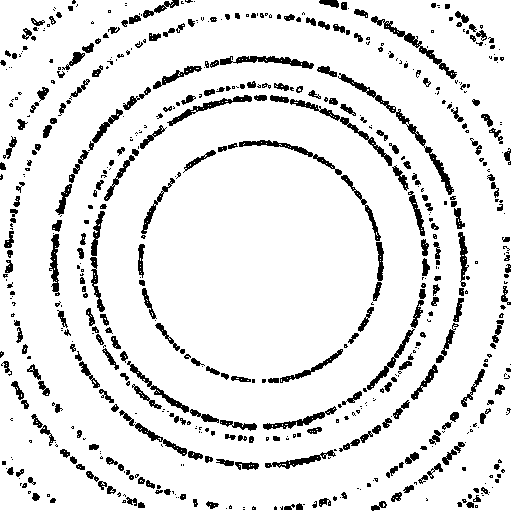
\includegraphics[width=\linewidth]{Detail/NorSmoothFull.png}&
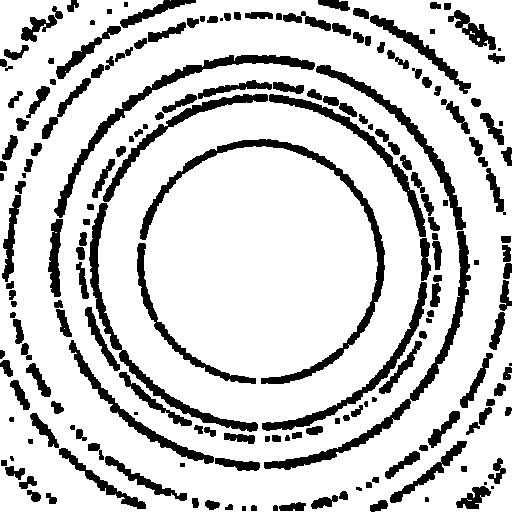
\includegraphics[width=\linewidth]{Detail/DilatedFull.png}&
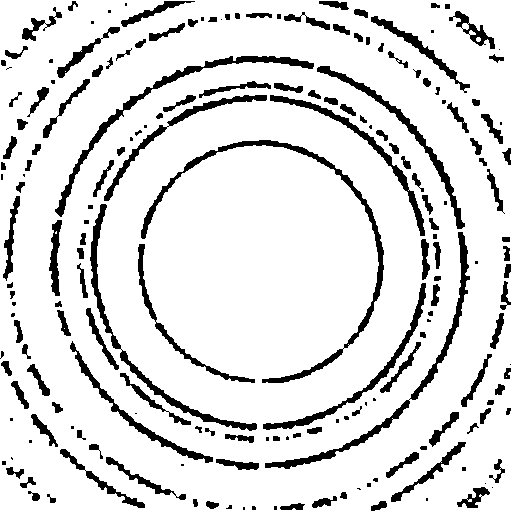
\includegraphics[width=\linewidth]{Detail/ThinnedFull.png}
\\
Zoomed in regions&

\includegraphics[width=\linewidth]{Detail/NorSmooth.png}&

\includegraphics[width=\linewidth]{Detail/Dilated.png}&

\includegraphics[width=\linewidth]{Detail/Thinned.png}
\\
Grown regions (Zoomed in)&
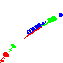
\includegraphics[width=\linewidth]{Detail/o_max1_Regs_Zin_Smooth.png}& &
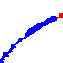
\includegraphics[width=\linewidth]{Detail/o_max1_Regs_Zin_thin.png}
\\
Grown regions (Full size)&
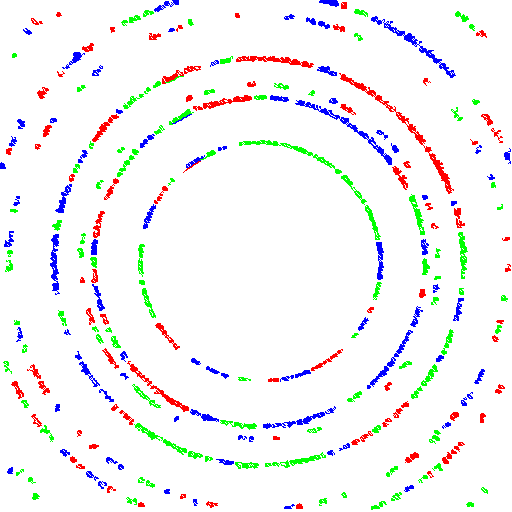
\includegraphics[width=\linewidth]{Detail/o_max1_Regs_aftr_norSmooth.png}& &
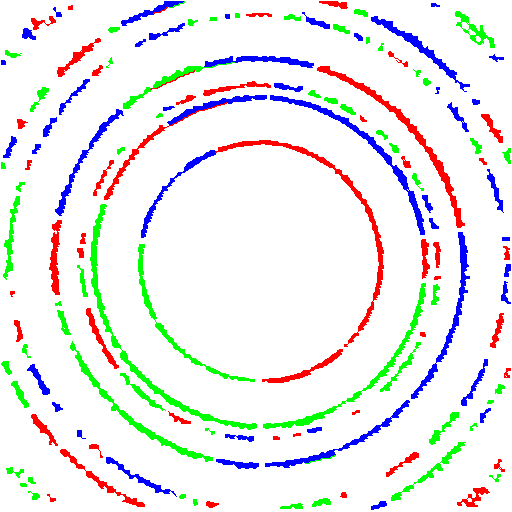
\includegraphics[width=\linewidth]{Detail/o_max1_Regs_aftr_thin.png}
\end{tabular}

\caption{Effect of morphological dilation and thinning on filling gaps within {\dsrs}. 
From above: The first row shows full size images, the second row shows a zoomed
in portion of one ellipse, the third row shows the grown region inside the
zoomed-in portion and the fourth row displays the full image after the
region-growth. Each colour represents a different region. Subsequent region
growing produces a much better picture than the original one, the gaps being
filled in by the present algorithm. The first column (\textbf{left}) shows the
original image, the second column shows the dilated image and the third shows
the final (thinned) image.}       

\label{fig:Dilt_Thin}
\end{figure}


This region growing algorithm is the one discussed in \cite{puatruaucean12A}.
An ordered list of pixels is obtained after the Gap Filling phase
(section-\ref{sec:gapFilling}). 
The logical status of each pixel is initially set to false, then we apply a
neighbourhood search algorithm for each pixel. 
Starting from a seed pixel, neighbour harvesting is performed by collecting
neighbouring pixels which have $almost$ the same orientation. 
Similarity in orientation is scored up to an angular threshold called $\tau$,
and each time this occurs, the status of selected neighbours toggles into true. 
Each selected neighbour is, in turn, further polled to find its neighbour
candidates. 

This search stops when no more neighbours exist whose gradient orientation
difference with region-orientation is lower than or equal to $\tau$.
The selected pixels are labelled as one region.
This region is generally referred as $R$.
This search is repeated for all pixels whose status is false, taking each of
them as a seed pixel one by one. 
In the present algorithm, since we are in quest of elliptic regions, we set
$\tau$ equals 45 degree. 

\subsection{Incremental Ellipse Detection (IED)} \label{subsec:EllipseGrow}
Once regions corresponding to elliptical segments are found, we can merge
multiple constituent regions to capture valid ellipses. 
However, which regions to merge is not known, a priori.
Given correct regions, ellipse fitting is easy and, conversely, given a correct
ellipse, finding its constituent regions is also easy. 
However, in our case, neither the ellipse nor the constituent regions are known.
Therefore, we fit ellipses in an incremental fashion as demonstrated in Figure
\ref{fig:working}. 
We start with the largest region (shown in blue) and fit an ellipse (in green)
to it. 
Then, we find other new regions (in red) that lie close to the current (blue)
region as well as the fitted (green) ellipse and add them to the current region.  
A new ellipse is fitted to this enlarged region and the process is repeated
until convergence. 
We iteratively apply the same procedure to the next largest unclaimed region.


\begin{figure}
\centering

\begin{tabular}{>{\centering\arraybackslash}m{.12\linewidth}
>{\centering\arraybackslash}m{.19\linewidth}
>{\centering\arraybackslash}m{.19\linewidth}
>{\centering\arraybackslash}m{.19\linewidth}
>{\centering\arraybackslash}m{.19\linewidth}}    

&Iteration 1 & Iteration 2 & Iteration 3 & Iteration 4
\\
{\color{blue}Region}&
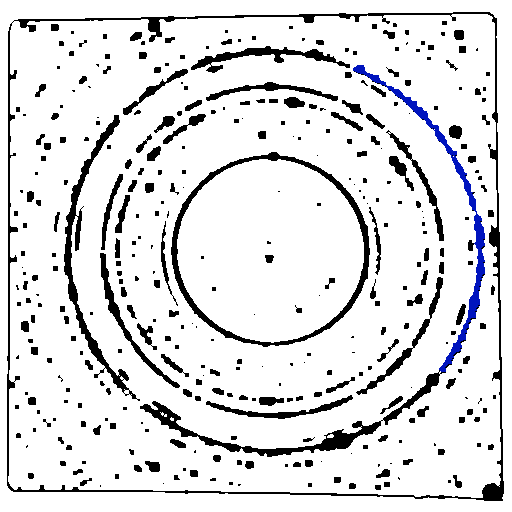
\includegraphics[width=\linewidth]{Detail/o_Si12_0002_R_2_0.png}&
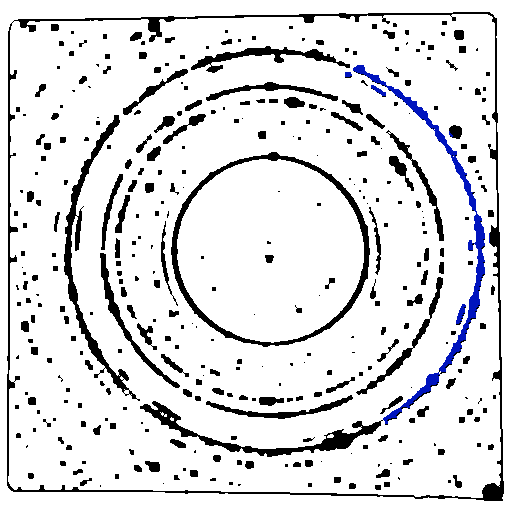
\includegraphics[width=\linewidth]{Detail/o_Si12_0002_R_2_1.png}&
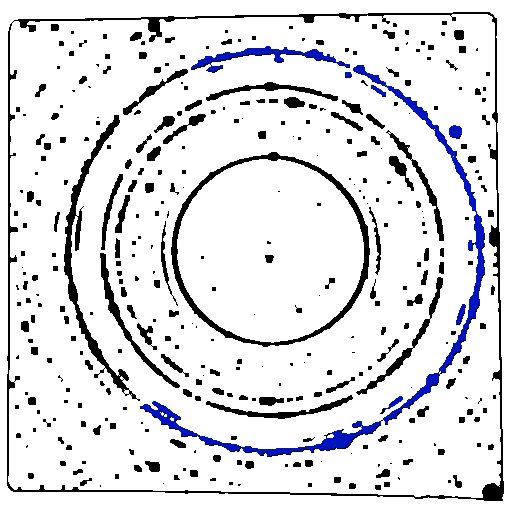
\includegraphics[width=\linewidth]{Detail/o_Si12_0002_R_2_2.png}&
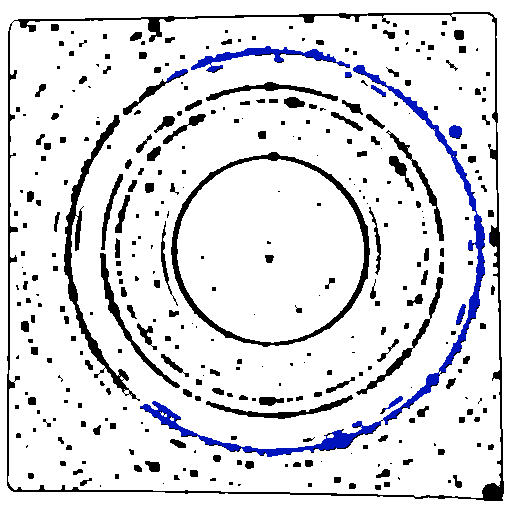
\includegraphics[width=\linewidth]{Detail/o_Si12_0002_R_2_3.png}
\\
{\color{green}Ellipse}&
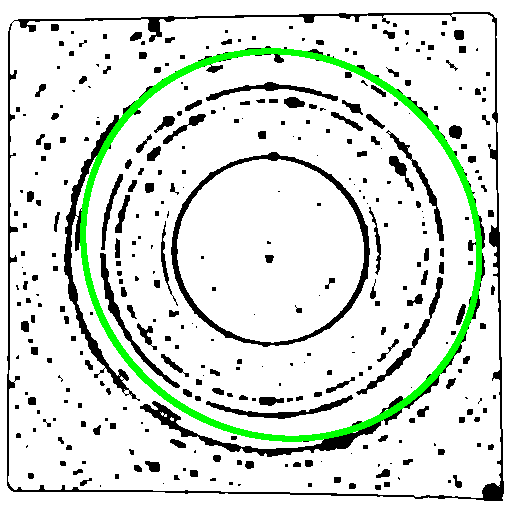
\includegraphics[width=\linewidth]{Detail/o_Si12_0002_E_2_0.png}&
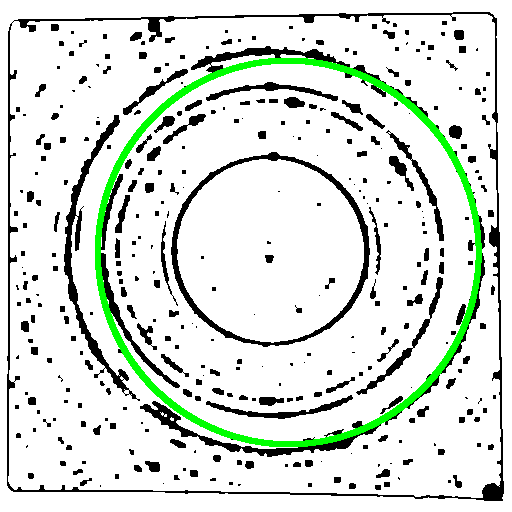
\includegraphics[width=\linewidth]{Detail/o_Si12_0002_E_2_1.png}&
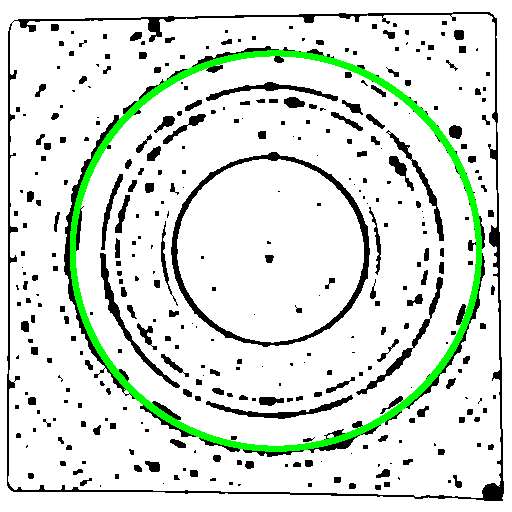
\includegraphics[width=\linewidth]{Detail/o_Si12_0002_E_2_2.png}&
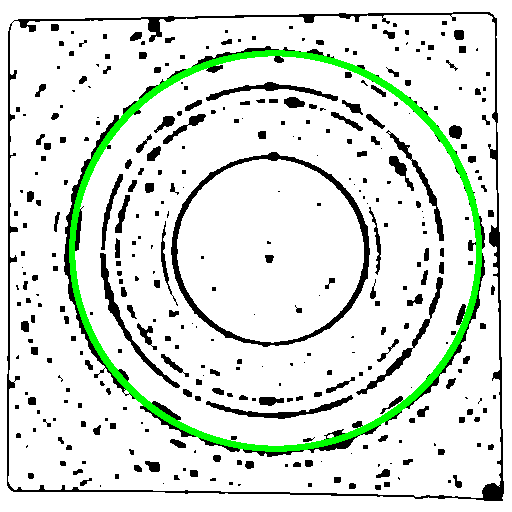
\includegraphics[width=\linewidth]{Detail/o_Si12_0002_E_2_3.png}
\\
{\color{red}Neighbouring Regions}&
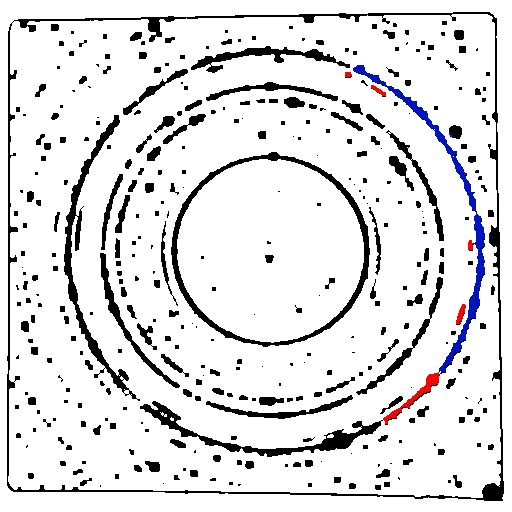
\includegraphics[width=\linewidth]{Detail/o_Si12_0002_DR_2_1.png}&
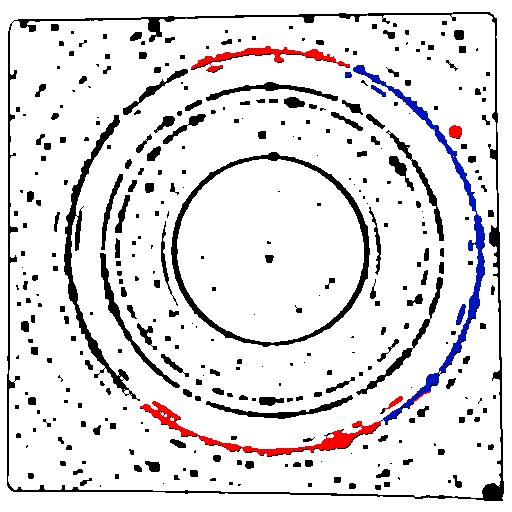
\includegraphics[width=\linewidth]{Detail/o_Si12_0002_DR_2_2.png}&
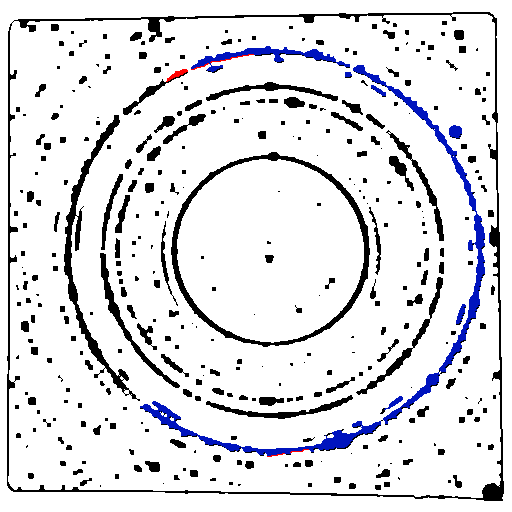
\includegraphics[width=\linewidth]{Detail/o_Si12_0002_DR_2_3.png}&
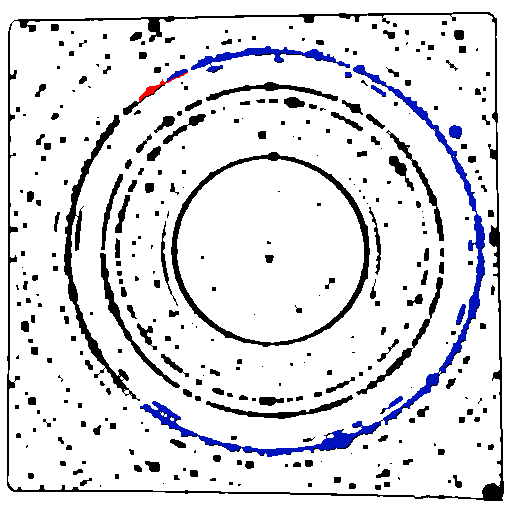
\includegraphics[width=\linewidth]{Detail/o_Si12_0002_DR_2_4.png}

\\&Iteration 5 & Iteration 6 & Iteration 7 & Converged
\\

{\color{blue}Region}&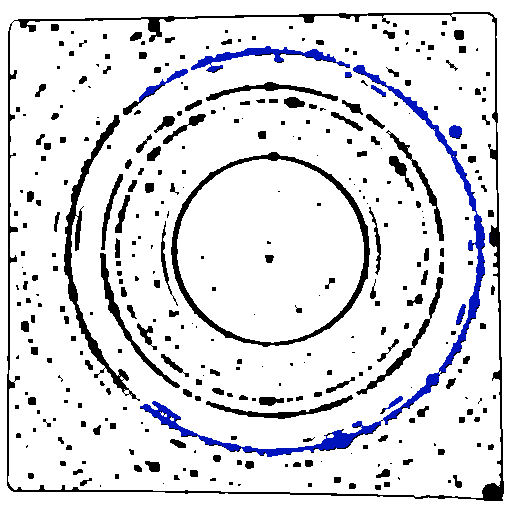
\includegraphics[width=\linewidth]{Detail/o_Si12_0002_R_2_4.png}&
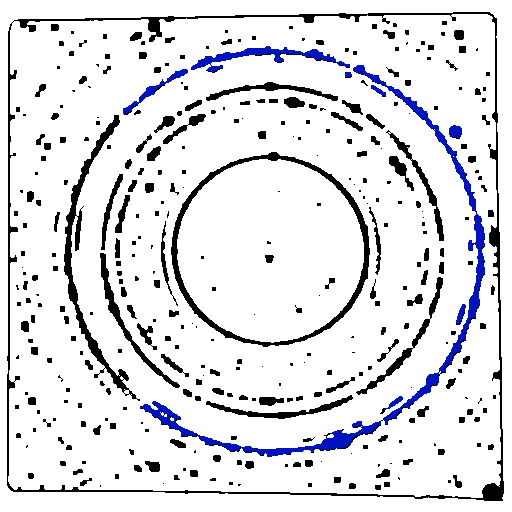
\includegraphics[width=\linewidth]{Detail/o_Si12_0002_R_2_5.png}&
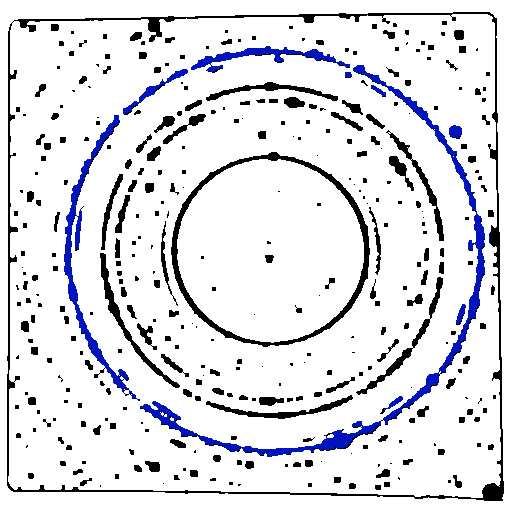
\includegraphics[width=\linewidth]{Detail/o_Si12_0002_R_2_6.png}&
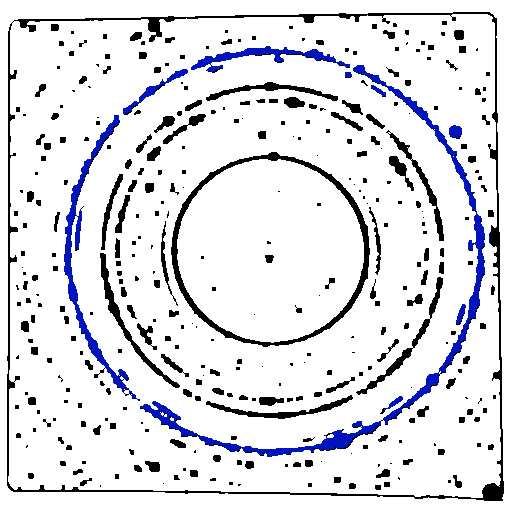
\includegraphics[width=\linewidth]{Detail/o_Si12_0002_RF_2_7.png}
\\
{\color{green}Ellipse}&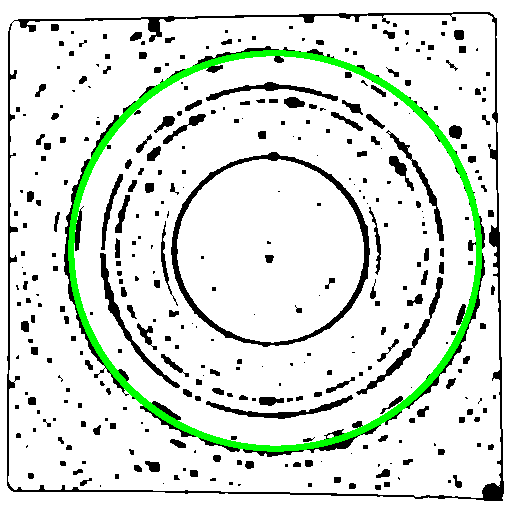
\includegraphics[width=\linewidth]{Detail/o_Si12_0002_E_2_4.png}&
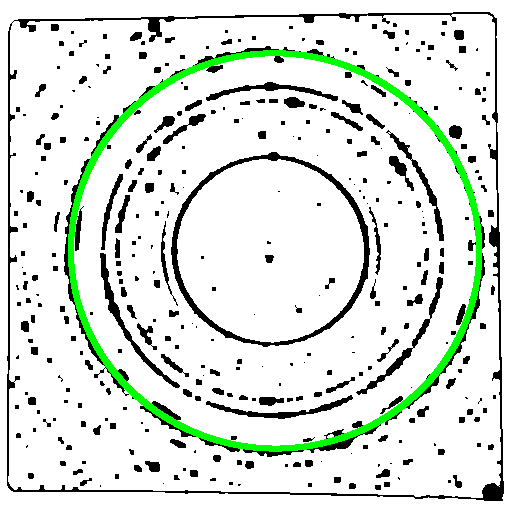
\includegraphics[width=\linewidth]{Detail/o_Si12_0002_E_2_5.png}&
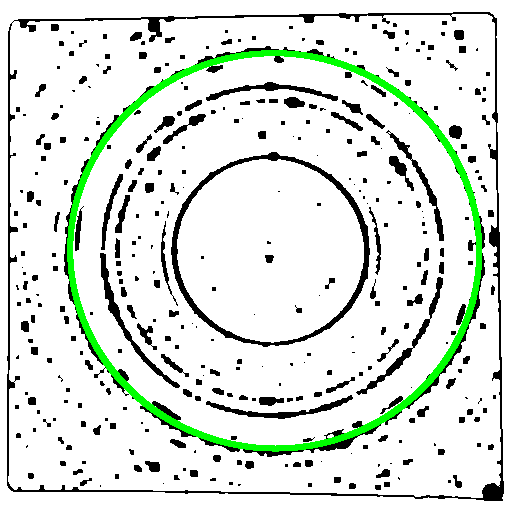
\includegraphics[width=\linewidth]{Detail/o_Si12_0002_E_2_6.png}&
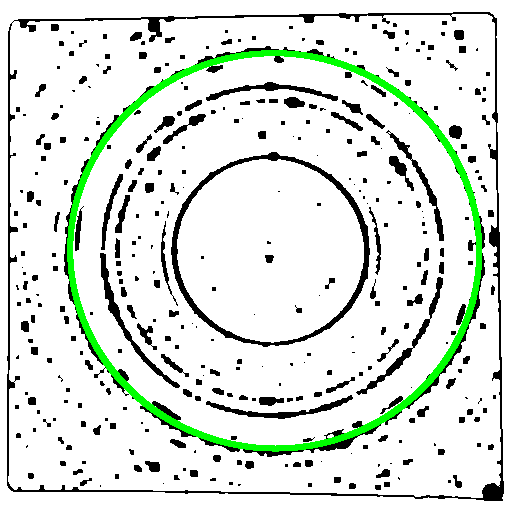
\includegraphics[width=\linewidth]{Detail/o_Si12_0002_EF_2_7.png}
\\
{\color{red}Neighbouring Regions}&
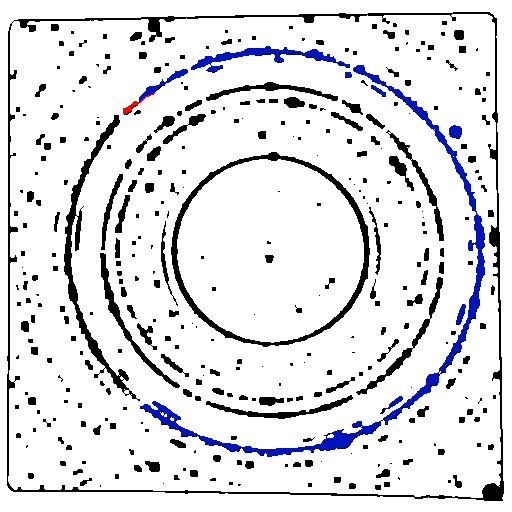
\includegraphics[width=\linewidth]{Detail/o_Si12_0002_DR_2_5.png}&
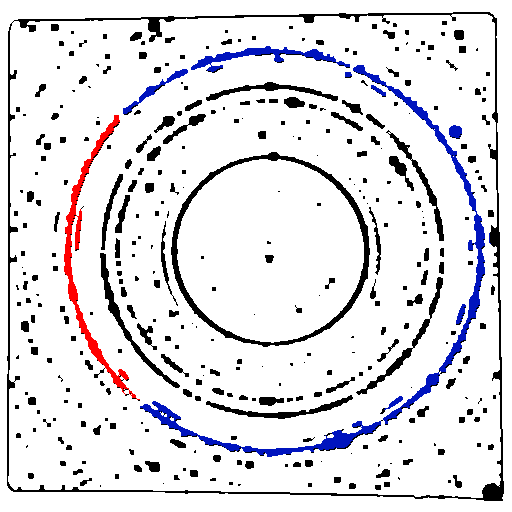
\includegraphics[width=\linewidth]{Detail/o_Si12_0002_DR_2_6.png}&
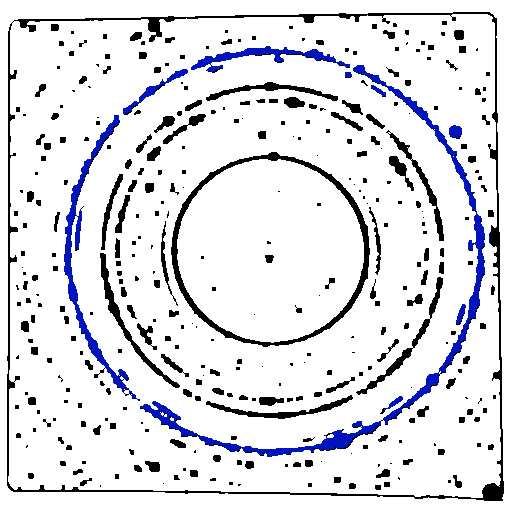
\includegraphics[width=\linewidth]{Detail/o_Si12_0002_R_2_6.png}&
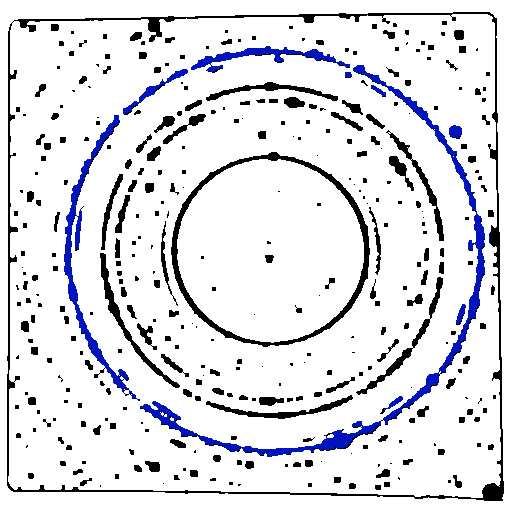
\includegraphics[width=\linewidth]{Detail/o_Si12_0002_RF_2_7.png}
\end{tabular}
\caption{Incremental ellipse detection (IED). 
From above: the first row of each iteration shows the current region (in blue). 
The second row shows the ellipse fitted to this region (in green) and the third
row shows neighbouring regions (in red) close to the current region and the
ellipse. The columns from \textbf{left} to \textbf{right} show successive
iterations.   
The neighbouring regions are merged into the current region for the next ellipse
fitting iteration until convergence is reached.} 

\label{fig:working}
\end{figure}

The algorithm flowchart is illustrated in Figure \ref{fig:flowChart}.

%In our case, we don't have prior knowledge of which subset of regions/segments belongs to a particular ellipse. 

\tikzstyle{startstop} = [rectangle, rounded corners, minimum width=3cm, minimum height=1cm,text centered, draw=black, fill=red!30]

\tikzstyle{io} = [trapezium, trapezium left angle=70, trapezium right angle=110, minimum width=2cm, minimum height=1cm, text centered, draw=black, fill=blue!30]

\tikzstyle{process} = [rectangle, minimum width=5cm, minimum height=1cm, text centered, draw=black, fill=orange!30, text width=4cm]
\tikzstyle{decision} = [diamond, minimum width=3cm, minimum height=3cm, text centered, draw=black, fill=green!30, text width=3cm]

\tikzstyle{arrow} = [thick,->,>=stealth]

\begin{figure}
\centering
\scalebox{.58}{
\begin{tikzpicture}[node distance=2cm]

%<TikZ code>
\node (start) [startstop] {Start};

\node (pPreProc) [process, right of=start, xshift=2cm, minimum width=3cm, text width=2cm] {Gap Filling};%{Preprocessing};
\node (pRegGrow) [process, right of=pPreProc, xshift=2cm, minimum width=3cm, text width=2cm] {Region Growing};

\node (dOuter) [decision, below of=pRegGrow, yshift=-1.5cm] {WHILE (Unclaimed Regions exist)};

\node (pO1) [process, below of=dOuter, yshift=-2cm] {Set next Region to current Region};

\node (pO2) [process, below of=pO1] {Fit Ellipse to Current Region};

\node (dInner) [decision, below of=pO2, yshift=-1.5cm] {WHILE (Current ellipse is not good};

\node (pI1) [process, below of=dInner, yshift=-2cm] {Select neighbours close to this region};

\node (pI2) [process, below of=pI1, yshift=-1cm] {Select neighbours from above selection which are close to current ellipse};

\node (pI3) [process, below of=pI2, yshift=-1cm] {Add selected neighbours to current region};

\node (pI4) [process, below of = pI3] {Fit ellipse to current region};

\node (pO3) [process, right of=dInner, xshift=4cm] {Store ellipse parameters};

\node (pO4) [process, below of=pO3] {Store Region};

\node (pO5) [process, below of=pO4] {Select next region as current region};

\node (pShow) [process, left of=dOuter, xshift=-4cm] {Show Final Output};

\node (end) [startstop, below of=pShow] {End};

\draw [arrow] (start.east)    -- (pPreProc.west);
\draw [arrow] (pPreProc.east) -- (pRegGrow.west);
\draw [arrow] (pRegGrow) -- (dOuter);
\draw [arrow] (dOuter)   -- node[anchor=east] {true} (pO1);
\draw [arrow] (dOuter)   -- node[anchor=south] {false} (pShow);

\draw [arrow] (pO1)      -- (pO2);
\draw [arrow] (pO2)      -- (dInner);
\draw [arrow] (dInner)   -- node[anchor=east] {true} (pI1);
\draw [arrow] (dInner)   -- node[anchor=south] {false} (pO3);

\draw [arrow] (dInner)   -- (pI1);
\draw [arrow] (pI1)      -- (pI2);
\draw [arrow] (pI2)      -- (pI3);
\draw [arrow] (pI3)      -- (pI4);
\draw [arrow] (pO3)      -- (pO4);
\draw [arrow] (pO4)      -- (pO5);
\draw [arrow] (dOuter)   -- (pShow);
\draw [arrow] (pShow)    -- (end);

\draw [arrow] (pO5.east) -| ++(2,0) |- (dOuter.east);
\draw [arrow] (pI4.west) -| ++(-2,0) |- (dInner.west);

\end{tikzpicture}
}
\caption{Flowchart of the IED algorithm.}
\label{fig:flowChart}
\end{figure}
\pagebreak


\section{Ellipse Evaluation} \label{sec:ellipseEval}
In the present context, ellipse evaluation means finding the fitness of an
ellipse. 
Instead of just visual analysis, we have devised an evaluation method to
numerically check the quality of fitted ellipses. 
The following sections describe the measures for ellipse evaluation and the
criteria based on these measures. 

\subsection{Ellipse Evaluation Measures} \label{sec:evalMeasures}
In order to accept or reject an ellipse and then rank all accepted ellipses, we
use following two evaluation measures. 
Both measures depend upon set of points $R$ on which ellipse $E$ is fit, and set
of points lying on the boundary of ellipse $E$ are generated via parametric
representation of ellipse.  

\subsubsection{Percentage of claimed angles.}
In order to estimate the fitness score of an ellipse, the angular coverage of an
ellipse $E$ by the region $R$ is measured. 
More coverage means greater fitness.
Total angles of ellipse are 360.

$x_i$ is a 2D point in a region $R$, $\alpha_i$ is a scalar representing the
angle subtended at point $x_i$. 
If A(R) represent set of unique angles $\alpha_i$ claimed by all the points in
region $R$. 
$\hat{x}_i$ is a 2D point on the boundary of the ellipse $E$ at an angle $\alpha
\in A(R)$. 
$v(\hat{x}_\alpha)$ is true (=1) if point $v(\hat{x}_\alpha)$ viewable in the
image and false(=0) otherwise. 

\begin{align}
v(x) = 
\begin{cases}
      1, & \text{if viewable}\  \\
      0, & \text{otherwise}
\end{cases}      
\end{align}


\begin{figure}
\centering
\begin{tabular}{c}
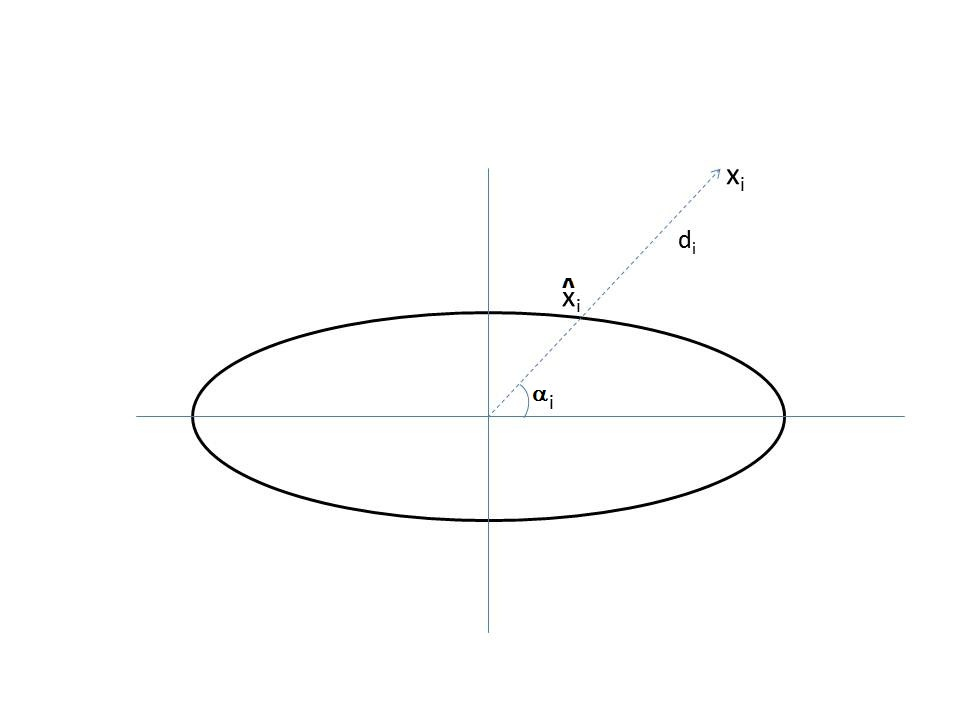
\includegraphics[width=.8\linewidth]{Figures/Ellipse_fig_new1.jpg}     
\end{tabular}
\caption{Ellipse with region point $x_i$, angle $\alpha_i$ and boundary point
$\hat{x}_i$ on the ellipse.} 
\label{fig:ellipse}
\end{figure}

\begin{equation} \label{eq:cap}
    \mathcal{C}(R,E) = \frac{\sum_{\alpha \in A(R)} v(\hat{x}_\alpha)} {\sum_{\alpha = 1}^{360} v(\hat{x}_\alpha)} * 100
\end{equation}

where the numerator counts the total number of unique angles of ellipse $E$ that
are claimed by the points in region $R$. 
Hence, the summation in the denominator of Equation (\ref{eq:cap}) is the total
number of viewable points on ellipse $E$. 

Figure \ref{fig:cap} shows $\mathcal{C(R,E)}$ values for the $(R, E)$ pairs as
the region is incrementally grown. 
It can be seen that the $\mathcal{C(R,E)}$ value is small when the region is not
full elliptical shape and large when the region covers an entire ellipse. 

\begin{figure}
\centering
\begin{tabular}{>{\centering\arraybackslash}m{.1\linewidth}>{\centering\arraybackslash}m{.25\linewidth}>{\centering\arraybackslash}m{.25\linewidth}>{\centering\arraybackslash}m{.25\linewidth}}
{\color{blue}Region}&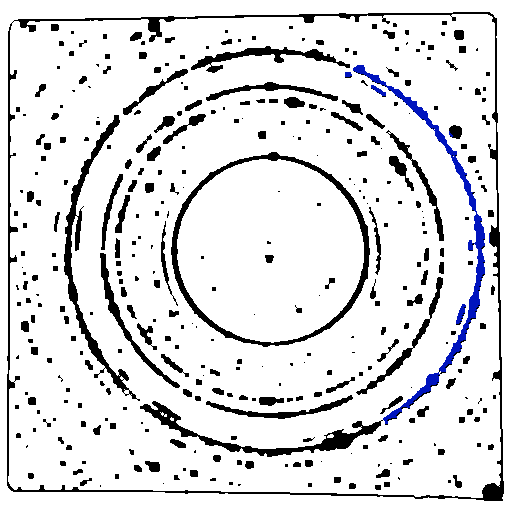
\includegraphics[width=\linewidth]{Detail/o_Si12_0002_R_2_1.png}&
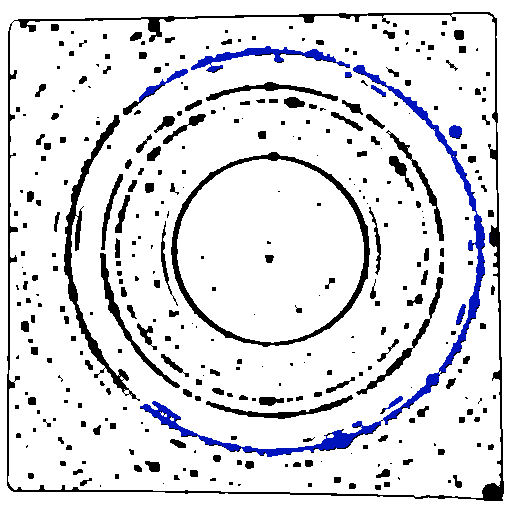
\includegraphics[width=\linewidth]{Detail/o_Si12_0002_R_2_4.png}&
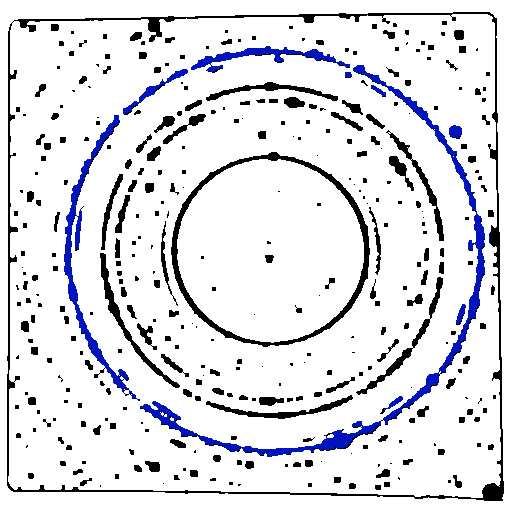
\includegraphics[width=\linewidth]{Detail/o_Si12_0002_R_2_6.png}
\\
{\color{green}Ellipse}&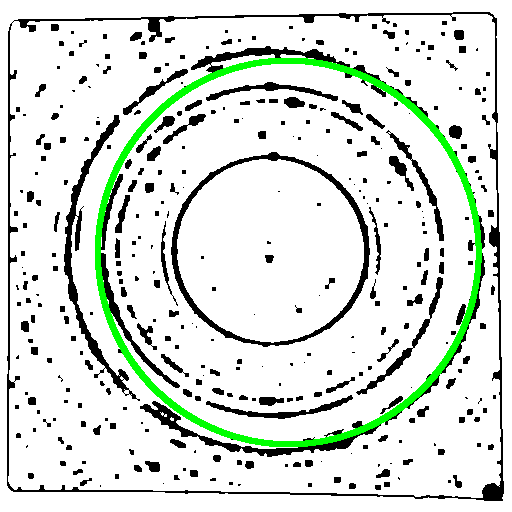
\includegraphics[width=\linewidth]{Detail/o_Si12_0002_E_2_1.png}&
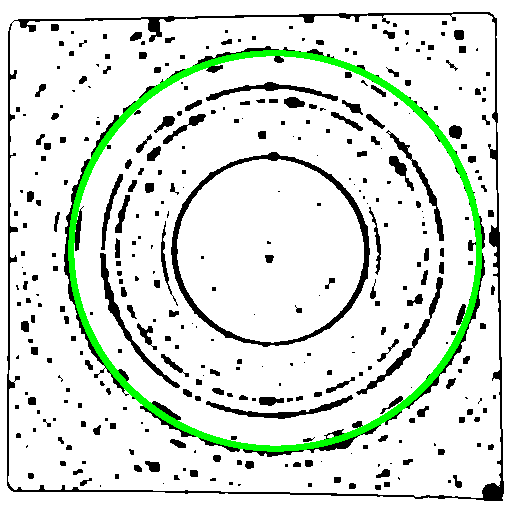
\includegraphics[width=\linewidth]{Detail/o_Si12_0002_E_2_4.png}&
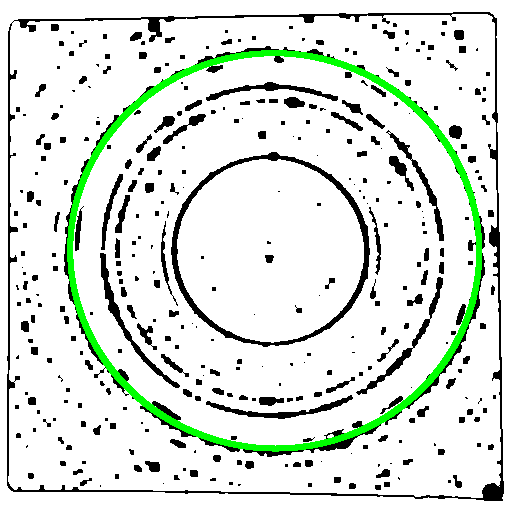
\includegraphics[width=\linewidth]{Detail/o_Si12_0002_E_2_6.png}
\\
$\mathcal{C}$& 37\% & 73\% & 100\%
\end{tabular}
\caption{Claimed angle percentage $\mathcal{C(R,E)}$ as $R$ and $E$ are
incrementally grown. 
As the region becomes more elliptical, the percentage of claimed angles
increases.} 
\label{fig:cap}
\end{figure}

\subsubsection{Average points-to-ellipse distance.}
Average distance of points in region $R$ to the ellipse $E$ is a measure to
assess the goodness of fit. 
For each point $x_i$ in the region $R$, we measure its geometric distance $d_i$
to the nearest point $\hat{x}_i$ on the boundry of ellipse $E$, i.e.
$d_i$=$\norm{x_i - \hat{x}_i}$.  
Then, we compute the average of such distances as:
\begin{equation} \label{eq:ADE}
    \mathcal{D}(R,E) = \frac{1}{\lvert R \rvert}  \sum_{i \in R} \norm{x_i -
    \hat{x}_i} 
\end{equation}

Figure \ref{fig:ade} displays the values for $\mathcal{D}(R,E)$ for three
different $(R, E)$ pairs. 
It can be seen that the value is large for poor ellipse fits and small for good
ellipse fits. 
\begin{figure}
\centering

\begin{tabular}{>{\centering\arraybackslash}m{.1\linewidth}>{\centering\arraybackslash}m{.25\linewidth}>{\centering\arraybackslash}m{.25\linewidth}>{\centering\arraybackslash}m{.25\linewidth}}
{\color{blue}Region}&
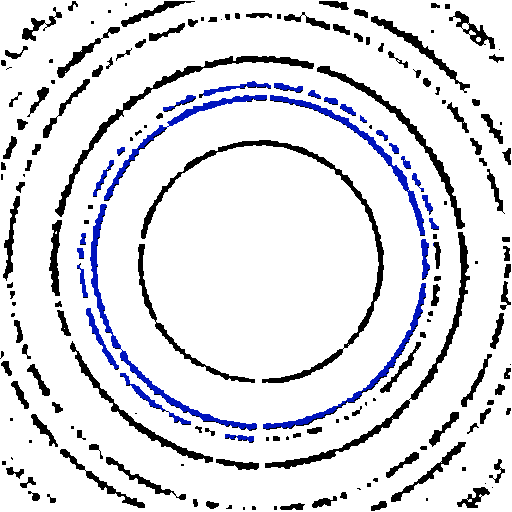
\includegraphics[width=\linewidth]{Detail/o_max1_RF_1_6.png}&
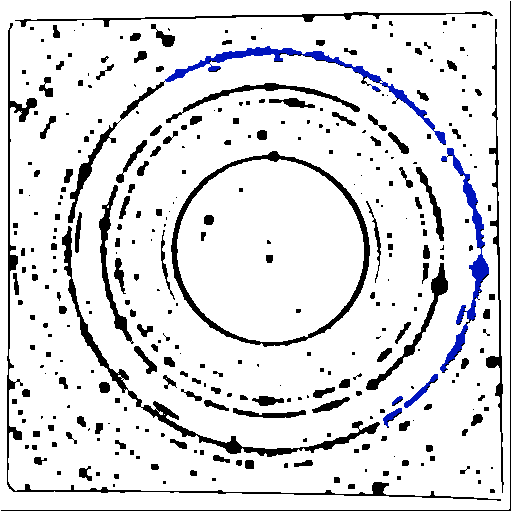
\includegraphics[width=\linewidth]{Detail/o_Si12_0001_RF_2_6.png}&
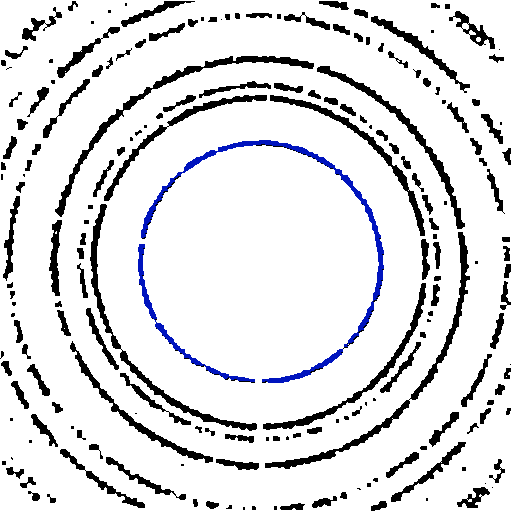
\includegraphics[width=\linewidth]{Detail/o_max1_RF_2_5.png}
\\
{\color{green}Ellipse}&
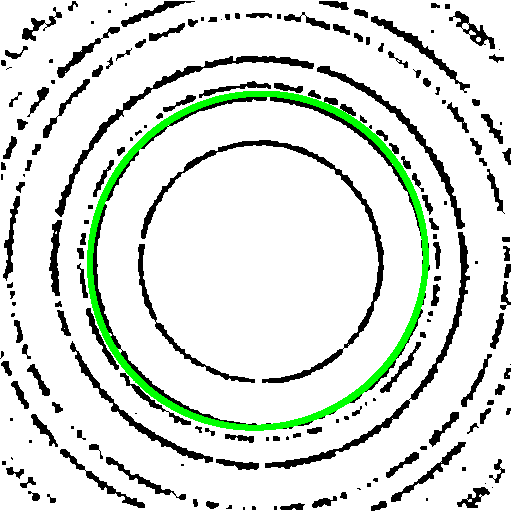
\includegraphics[width=\linewidth]{Detail/o_max1_EF_1_6.png}&
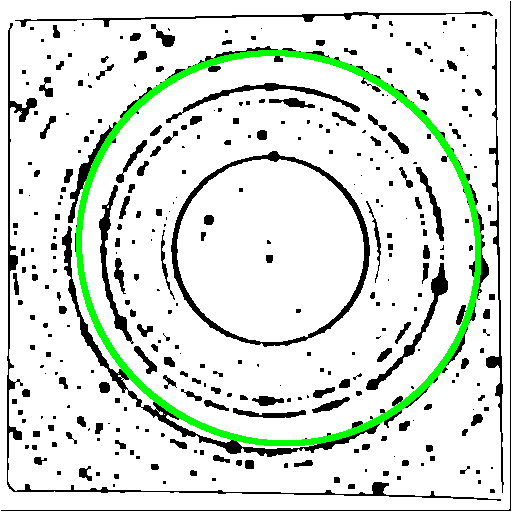
\includegraphics[width=\linewidth]{Detail/o_Si12_0001_EF_2_6.png}&
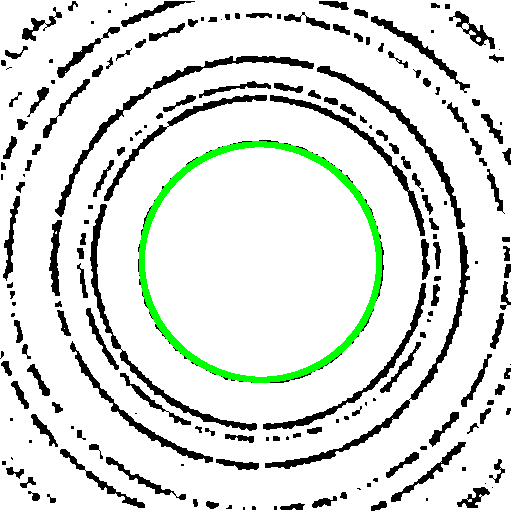
\includegraphics[width=\linewidth]{Detail/o_max1_EF_2_5.png}
\\
$\mathcal{D}$ & $5.25$ pixels & $2.63$ pixels & $1.43$ pixels
\end{tabular}

\caption{Average $\mathcal{D}$ (i.e. distance to ellipse) values for three
different $(R, E)$ pairs. It can be seen that the value is large for poor
ellipse fits and small for good ellipse fits and is therefore a measure of
closeness between the region and the fitted ellipse.}   

\label{fig:ade}
\end{figure}

\subsection{Ellipse Evaluation Criteria}  \label{sec:evalCriteria}
We use measures of $\mathcal{C}(R,E)$ and $\mathcal{D}(R,E)$, as described in
Section \ref{sec:evalMeasures} to evaluate the ellipses at certain stages of the
IED algorithm.  
The following sub-sections describe the use of these measures.
\subsubsection{Convergence Criteria}
Our ellipse growing algorithm is incremental and iteratively keeps on merging
regions to generate an ellipse until 
\begin{enumerate}
    \item the claimed angle percentage $\mathcal{C}(R,E)$ is greater than a
    threshold value ${\tau}_C$, or 
    \item no more candidate points for region $R$ are found.
\end{enumerate}

This helps in faster execution by stopping the ellipse growing process as soon
as an acceptable level of fitness is achieved. 

\subsubsection{Acceptance/Rejection Criteria}
After convergence, it is decided whether an ellipse is valid or not.
This is done by validating ellipses in the following three ways.
A grown ellipse is accepted if
\begin{enumerate}
    \item the claimed angle percentage $\mathcal{C}(R,E)$ is greater than or
    equal to a threshold ${\tau}_{C_{Min}}$, and 
    \item the average distance $\mathcal{D}$ to an ellipse is less than a
    threshold ${\tau}_D$, and 
    \item the length ratio between the major axis and the minor axis is less
    than a threshold ${\tau}_R$ 
\end{enumerate}

The last requirement prevents detection of extremely elongated ellipse
configurations. 

\subsection{Ranking of Ellipses}
Once all valid ellipses are found, it is useful to rank them so that subsequent
processing can be done at a high confidence level. 
Our ranking is based on $\mathcal{D}(R,E)$ (Equation (\ref{eq:ADE})).
The ranking is done by sorting all valid ellipses in ascending order based on
their distance values $\mathcal{D}(R,E)$. 
The ellipse with the lowest average $\mathcal{D}(R,E)$ value is ranked best. 

For all calculations in this paper, the threshold values were set as
${\tau}_C=90\%$, ${\tau}_{Cmin}=50\%$, ${\tau}_D=10$ and ${\tau}_{ratio}=2$. 

The proposed IED algorithm followed by the ranking algorithm provides good
results on images, overcoming various types of challenges. 
Common types of challenges with {\dsr} patterns are:

\begin{itemize}
    \item scattered data i.e. gaps along the rings
    \item partial ellipses (resulting from tilted detectors)
    \item noisy contours
    \item other artifacts like blobs etc.
\end{itemize}

Figure \ref{fig:result1} shows results from various types of challenging
patterns and demonstrates that our algorithms are able to detect ellipses. 
The numbers written next to the ellipses indicate the ranks of the respective
ellipses. 

\begin{figure}
\begin{tabular}{cc}

\includegraphics[width=.45\linewidth,height=.45\textheight,keepaspectratio]{Ranked/o_Si12_0002__Ranked.png}&
\includegraphics[width=.45\linewidth,height=.45\textheight,keepaspectratio]{Ranked/o_tilted_002__Ranked.png}
\end{tabular}

\begin{tabular}{cc}
\includegraphics[width=.95\linewidth,keepaspectratio]{Ranked/o_LaB6_0021__Ranked.png}
\end{tabular}

\label{fig:result1}
\caption {Moving clockwise from the \textbf{top-left} side, we can see two
ellipses in the \textbf{top-left} image (including the inner-most ring) in
presence of significant gaps and noisy contours along the rings. 
In the \textbf{top-right} image, although only partial ellipses are available,
still many valid ellipses are detected. 
In the \textbf{bottom} image, rings are too
close to each other and some blobs are also there, so not all automatically
detected ellipses are good (notice some falsely predicted ellipses).      
Still a number of good ellipses are detected.}
\end{figure}

There are two types of detector configuration; one is the detector which is
orthogonal to the incoming beam (orthogonal detector) and the other is one which
is not orthogonal (tilted detector).  
The next two sections (\ref{sec:removalFD} and \ref{sec:family}), propose two
refinements of results. 
These refinements are in case of orthogonal detectors only.

\section{Removal of False Detections}
\label{sec:removalFD}
As we can see in the last row of Figure \ref{fig:result1}, there are many
ellipses detected. 
Some ellipses are true and some are false detections.
These false detections occur because of noise in the image and/or very little
gap between two ellipses. 
In this section, we will describe how to remove these false detections.
This is done in two phases:
\begin{enumerate}
    \item Classification of images \emph{i.e.} whether an image comes from an
    orthogonal or a tilted detector. 
    \item Identification and removal of false ellipses in images from orthogonal
    detectors. 
\end{enumerate}

\subsection{Classification of images}
The false ellipse detections in  (Figure \ref{fig:result1}) belong to a frame
issued by an orthogonal detector only. 
We can easily classify whether a pattern comes from an orthogonal detector or a
tilted one by reviewing the parameters of the detected ellipses. 
One can see that \dsrs{} for orthogonal detectors are generally scaled versions
of each other. 
Therefore, their major-to-minor axis length ratios are very similar.
This allows us to mark any detected ellipse with a significantly different ratio
as a false detection. 

Specifically, the major-to-minor axis length ratio is recorded for all detected
ellipses. 
Then we compute a histogram of these ratios.
The centre of the histogram bin with maximum count is considered as the mode of
these ratios. 
By thresholding this mode value, we are able to decide whether a given image
results from an orthogonal or a tilted detector. 
The outliers are found and removed in images from orthogonal detectors only.

\subsection{Identification and removal of false detections}
By checking these outliers, we could clearly see that their centres are quite
dispersed and also far from centres of correct ellipses. 
In addition to, centres of correct ellipses are close to each other.
Thus, we want to find a representative centre $\mathbf{\bar{c}}$ which will
represent the centre of the correct ellipses. 
By finding the deviation of each ellipse centre from $\mathbf{\bar{c}}$, we can
classify whether an ellipse is an outlier or not. 
Finding this representative centre cannot be done using the mean value because
the mean is always sensitive to outliers and false ellipses' centres are quite
far-off from $\mathbf{\bar{c}}$.  

One might be tempted to use the median which is robust to outliers.
However, such robustness is only when there are relatively few outliers.
When the number of outliers approaches or exceeds the number of inliers, then
even the median does not remain robust. 

The mode is a good choice because, as stated earlier, the centres of outliers
are dispersed and the centres of correct ellipses are close to each other. 
We use a 2D histogram for finding the mode of the ellipse centres.
This mode centre, $\mathbf{\bar{c}}$, works as a representative centre for all
correct ellipses.  

After finding $\mathbf{\bar{c}}$, we calculate the Euclidean distance of all
ellipses' centres from it. 
By thresholding the Euclidean distance, our algorithm automatically decides
whether an ellipse is an outlier or a correct one. 
Figure \ref{fig:result_outliers} displays images before and after removal of
false detections. 

\begin{figure}
\begin{tabular}{c}
\includegraphics[width=.80\linewidth]{Outliers/o_LaB6_0021__Ranked_FullSize_9.png}
\\
\includegraphics[width=.80\linewidth]{Outliers/o_Lab6_0021__Ranked_FullSize_3.png}
\end{tabular}

\label{fig:result_outliers}
\caption {The \textbf{top} frame shows outliers before removal. 
The \textbf{bottom} frame shows the result after removing outliers. 
After removal, the remaining ellipses are ranked again according to their
correct telly ranking.} 
\end{figure}

\section{Refinement via Elliptical Family constraint}
\label{sec:family}
From the results shown so far, not all {\dsrs} are detected by our algorithm. 
Sometimes valid \dsrs{} are rejected since the detected corresponding ellipses
fail to pass all thresholds. 
This is a trade-off between correct and missing detections and cannot be avoided. 
Although calibration is possible from only a few rings, it is beneficial to
detect as many rings as possible. 
For this purpose we take a pure computer vision viewpoint, and note that {\dsrs}
can be seen as \emph{families} of ellipses. 
For orthogonal detectors, a family can be obtained from equally scaled versions
of the major and minor ellipse axes such that their ratio is preserved. 
Consider an ellipse
$\mathbf{e}_1=\left[e_{\bar{x}},e_{\bar{y}},e_{\theta},e_a,e_b\right]^T$ with
centre $(e_{\bar{x}},e_{\bar{y}})$, angle $e_\theta$ , half-major axis length
$e_a$ and half-minor axis length $e_b$.   
Its family members can be generated as
$\mathbf{e}_k=\left[e_{\bar{x}},e_{\bar{y}},e_{\theta},ke_a,ke_b\right]^T$ for
$k\in\mathbb{R}^+$.  
%\begin{equation}
%    \textbf{e}^{\prime} =\left[ \begin{array}{l}
%        e_{x_0} \\
%        e_{y_0} \\
%        e_{\theta}\\
%        ke_a \\
%        ke_b
%    \end{array}\right]
%\end{equation}
This ensures that all members share the same centre, angle and shape
(\emph{i.e.}, ratio of axis lengths $\frac{e_a}{e_b}$). 
Note that this definition is not suitable for non-orthogonal detectors. 
Therefore, we focus in this section on \dsrs{} obtained through orthogonal
detectors only. 

For every detected ellipse $\mathbf{e}$, the proposed refinement involves
generating boundary points $E_k$ corresponding to ellipses $\mathbf{e}_k$ for
different\footnote{$k\approx1$ is avoided to prevent duplicate detections.}
$k\in\mathbb{R}^+$.   
For each such ellipse, we find the set $R_k$ of \dsr{} pixels that intersect the
boundary $E_k$. 
Finally, the validity of set $R_k$ as a \dsr{} can be determined by thresholding
the ratio $\frac{|R_k|}{|E_k|}$. 
%distance measure $\mathcal{D}(R_k,E_k)$ from Equation \ref{eq:ADE}.

Large interval in scales may cause our algorithm to miss some available ellipses
because of unavailability of intersections. 
This problem can be avoided by using smaller interval between scales. 

It must be noted that such a refinement can produce redundant detections, hence
it is important to post-process the results. 
For this, we compare the geometric representations of ellipses.
Specifically, two ellipses $\mathbf{e}_1$ and $\mathbf{e}_2$ are considered
distinct if the absolute difference $|e_{1i}-e_{2i}|$ for any component
$i\in\lbrace \bar{x}, \bar{y}, \theta, a, b\rbrace$ is greater than the
corresponding threshold $\tau_i$.   
If all five absolute differences are within their thresholds, then only one out
of $\mathbf{e}_1$ and $\mathbf{e}_2$ is retained. 

\begin{figure}
\begin{tabular}{ll|l|l|l}
%first row for incremental ellipse detection (IED)

\rotatebox[origin=l]{90}{\textbf{\small{IED}}}

&
\includegraphics[width=.18\linewidth]{withoutRanks/o_max1__woRank.png}
&
\includegraphics[width=.18\linewidth]{withoutRanks/o_Si12_0002__woRank.png}
&
\includegraphics[width=.18\linewidth]{withoutRanks/o_tilted_000__woRank.png}
&
\includegraphics[width=.32\linewidth]{withoutRanks/o_LaB6_0021__woRank.png}

%\begin{comment}

% 2nd row for family
\\
\rotatebox[origin=l]{90}{\textbf{\small{Family}}}
\centering
&
\includegraphics[width=.18\linewidth]{Family/o_max1__Family.png}
&
\includegraphics[width=.18\linewidth]{Family/o_Si12_0002__Family.png}
&
\includegraphics[width=.18\linewidth]{Family/o_tilted_000__Family.png}
&
\includegraphics[width=.32\linewidth]{Family/o_LaB6_0021__Family.png}

% 3rd row for Merged and redundant removed
\\
\rotatebox[origin=l]{90}{\textbf{\small{Merged}}}
&
\includegraphics[width=.18\linewidth]{Merged/o_max1__Merged.png}
&
\includegraphics[width=.18\linewidth]{Merged/o_Si12_0002__Merged.png}
&
\includegraphics[width=.18\linewidth]{Merged/o_tilted_000__Merged.png}
&
\includegraphics[width=.32\linewidth]{Merged/o_LaB6_0021__Merged.png}

%\end{comment}
\end{tabular}

%\end{landscape}
\label{fig:family1}
\caption {Refinement via family constraint for the four different {\dsr} images.
\textbf{Top-row} shows results of the IED algorithm, \textbf{middle-row} shows
result of refinement via family constraint and the \textbf{bottom-row} shows the
merged results.}  

\end{figure}

Figure \ref{fig:family1} displays refinement steps on orthogonal detector
patterns using the family constraint. 
It can be noticed that the refinement procedure recovers almost all \dsrs{} that
could have been recovered manually. 
Since the constraint is valid for orthogonal detectors only, refinement results
for non-orthogonal detectors are obviously not so good and this is demonstrated
in Figure \ref{fig:family_tilted}.  

\begin{figure}
\centering
\begin{tabular}{cc}

\textbf{Before refinement} & \textbf{After refinement}
\\
\includegraphics[width=.35\linewidth,height=.45\textheight,keepaspectratio]{withoutRanks/o_tilted_006__woRank.png}
&
\includegraphics[width=.35\linewidth,height=.45\textheight,keepaspectratio]{Merged/o_tilted_006__Merged.png}
\end{tabular}

\label{fig:family_tilted}
\caption {Refinement via orthogonal family constraint is not very useful for
non-orthogonal detectors which yield highly eccentric \dsrs.} 
\end{figure}

\section{Comparisons}
\label{sec:compr}
\subsection{\textbf{Comparison with the method by Rajiv et al.}}
\label{sec:rajiv}
{The work of \cite{PDJ:8503397} extracts \dsrs{} for orthogonal detectors only
under rather restrictive assumptions using a modified Hough transform. 
Since a $5$D Hough transform for ellipse detection is computationally demanding,
the authors suggest to decompose the Hough transform in order to work in $1$D only. 
This is achieved by making the following restrictive assumptions
\begin{enumerate}
    \item All {\dsrs} share the same centre.
    \item The centre of the {\dsrs} has to be within the image.
    \item Centre of the ellipse has to be close to the centre of the image.
\end{enumerate}
In addition, their algorithm also depends on carefully chosen radii for \dsrs{}
and this selection of radii is not automatic. 
}

{By contrast, our algorithm does not make any of these restrictive assumptions
and does not use prior information of the sample or diffraction setup. 
Our algorithm is able to detect partial \dsrs{} with centres located outside the
image which is often the case when non-orthogonal detectors are used. 
Figure \ref{fig:compare_rajiv} compares the result of our algorithm on two of
the images used by this method \cite{PDJ:8503397}. 
Our algorithm was able to detect all the {\dsrs} available in the image.
}

\begin{figure}
\centering
\begin{tabular}{cc}
\textbf{Sample Image} & \textbf{This work}
\\
\includegraphics[width=.35\linewidth]{Comparisons/rajiv1.png}
&
\includegraphics[width=.35\linewidth]{Comparisons/rajiv1OurResult.png}
\\
\includegraphics[width=.35\linewidth]{Comparisons/rajiv2.png}
&
\includegraphics[width=.35\linewidth]{Comparisons/rajiv2OurResult.png}
\end{tabular}

\label{fig:compare_rajiv}
\caption {Comparison with the method by Rajiv et. al.
Our algorithm recognises a number of ellipses higher than \cite{PDJ:8503397}. 
As we could work only on the imaeges from the PDF file of Rajiv et. al. paper,
we had to adapt slightly our pre-processing to it.} 
\end{figure}

\subsection{\textbf{Comparison with the method by Cervellino et. al.}}
\label{sec:cerv}
The authors in \cite{cervellino2006folding}, describe a method to identify
ellipses with \dsrs{} imposing the following two constraint: 

\begin{enumerate}
    \item Images should be taken from an(almost) orthogonal detector.
    \item The sample-to-detector distance should be known.
\end{enumerate}

The ellipses resulting from such detectors are nearly circular; and most of the
ellipses are available in the images they show. 
The algorithm we propose can work for orthogonal as well as for tilted detectors
and does not use any sample-specific parameter. 

\begin{figure}
\centering
\begin{tabular}{ccc}

\textbf{Sample Image} & \textbf{\cite{cervellino2006folding}} & \textbf{This work}
\\
\includegraphics[width=.30\linewidth]{Comparisons/fold1.png}
&
\includegraphics[width=.30\linewidth]{Comparisons/fold1CervResult.png}
&
\includegraphics[width=.30\linewidth]{Comparisons/fold1OurResult.png}
\end{tabular}

\label{fig:compare_cerv}
\caption {Comparison with the method by Cervellino et. al.
Our result contains a higher number of ellipses.}
\end{figure}

Figure \ref{fig:compare_cerv} compares results of method by
\cite{cervellino2006folding} with result of our proposed method on two {\dsr}
images.  
Our algorithm was able to detect all the {\dsrs} available in the image.

\section{Conclusion}
We proposed a new ellipse detection method which is specialised in the automatic
detection of \dsrs{} in 2D XRPD patterns. 
This method, provides a mechanism to detect complete and/or partial ellipses in
a given image. 
The first part of our algorithm, called incremental ellipse detection, groups
connected contours to find smaller elliptic arcs. 
Then, it gradually generates full ellipses by grouping unconnected elliptic arcs
in an incremental way. 
The initial results are refined by detecting families of found ellipses and
exploiting the family constraint. 
We not only devise an ellipse-detection method, we also provide a measure for
evaluating the goodness of the fit. 
Every fitted ellipse is evaluated based on the angular coverage of the fitted
portion/part and on the average distance of neighbouring points to the fitted
ellipse.
 Using this method, \dsrs{} can be detected automatically, dramatically
 accelerating the calibration of batches of  diffraction images. 
\dsr{} patterns, from tilted detectors, are not always ellipses.
They could be in some special cases, hyperbolae or parabolae.
In the forth coming study, we will show how we cope with this particular
problem. 

The matlab code is available at: \ldots

%\section{Acknowledgements}
\ack{Acknowledgements:}
The authors would like to thank the LinkSCEEM European program in the frame of  
this collaboration was initiated. 
 

%\section{References}
\bibliographystyle{iucr}
\bibliography{biblio}

\pagebreak
\appendix \textbf{Appendix A : Incremental Ellipse Detection Algorithm}
%\section{Algorithm}

\begin{algorithm}
\begin{algorithmic}[1]
\Procedure{IncrementalEllipseDetection}{}
\Comment{Detect ellipses via incremental region and ellipse improvement}

%\INPUT
\Statex R$_\text{initial}$, \Comment regions returned by \textsc{RegionGrow}

%\OUTPUT
\Statex $\text{E}_\text{final}$ \Comment{valid fitted ellipses}
\Statex $\text{R}_\text{final}$ \Comment{regions corresponding to fitted
ellipses}  
\Statex $\mathcal{C}_\text{final}$ \Comment{claimed angle percentages for each
ellipse-region pair} 
\Statex $\mathcal{D}_\text{final}$ \Comment{average point to ellipse distances
for each ellipse-region pair} 
\Statex $\text{ranking}$ \Comment{ranking of fitted ellipses}

%\State $\text{test\_points} \gets \text{all points of all regions}$
\State $\text{eNum} \gets 1$
\State $\text{UR} \gets \text{R}_{initial}$

\While {$\text{UR}\neq\emptyset$}

	\State $\text{CR} \gets \text{largest unclaimed region}$
	\State $\text{CE} \gets \textsc{FitEllipse}(\text{CR})$
	\State $[\mathcal{C}, \mathcal{D}] \gets \textsc{EvaluateEllipse}(\text{CR},
	\text{CE})$ 
	

	\While {$(\mathcal{C} < \tau_{\mathcal{C}})$}
	    
	 	\State $\text{N} \gets \textsc{GetRegionNeighbours}(\text{CR},
	 	\text{R}_\text{initial})$ 
		
    	\State $\text{N} \gets \textsc{GetEllipseNeighbours}(\text{CE},\text{N})$
		
%        \If {$\text{N}\neq\emptyset$}
            \State $\text{CR} \gets \text{CR}\cup\text{N}            $
%        \EndIf
        
		\State $\text{CE} \gets \textsc{FitEllipse}(\text{CR})$
		
		\State $[\mathcal{C}, \mathcal{D}] \gets \textsc{EvaluateEllipse}(\text{CR},
		\text{CE})$ 
	\EndWhile

   	\State $\text{E}_\text{final} \gets \text{E}_\text{final} \cup \text{CE}$
	\State $\text{R}_\text{final} \gets \text{R}_\text{final} \cup \text{CR}$
    \State $\mathcal{C}_\text{final} \gets \mathcal{C}_\text{final} \cup \mathcal{C}$
    \State $\mathcal{D}_\text{final} \gets \mathcal{D}_\text{final} \cup \mathcal{D}$
%	\State $\text{final\_\mathcal{D}[eNum]} \gets \mathcal{D}$
%	\State $\text{eNum} \gets \text{eNum} + 1$
	\State $\text{UR} \gets \text{UR} \setminus \text{CR}$
\EndWhile

%  \State \textbf{return} $final\_ellipses$\Comment{The Ellipse Parameter List}
\State $\text{ranking} \gets \textsc{sort}(\mathcal{D}_\text{final},\text{ascending})$
\EndProcedure
\end{algorithmic}
\caption{Incremental Ellipse Detection (IED). 
\memonazar{I have updated the algorithm.}} 
\label{alg:ied}
\end{algorithm}

%-------------------------------------------------------------------------
     % The back matter of the paper - acknowledgements and references
     %-------------------------------------------------------------------------

     % Acknowledgements come after the appendices





\begin{comment}
\section{ToDo List}


ToDO list include:

1)
Study and comparison of hyperbola vs. parabola : done - decided to take it as parabola
Finding parameters of parabola  : done - found formulas and calculations for vertex, focus and focal_length 
Plotting parabola  in-progress.  value of focal-Length is too small which causes problems in plotting. Not enough values of x.

2)
Merging of two sets of ellipses found (one from IED and 2nd from family of ellipses). Merging of sets includes removal of redundant ellipses i.e. finding unique set of ellipses. 

3) 
Why lines appear in pre-processing? Effect of gradients

4)
fig of ellipse : done

5) 
Correcting any alignment / spacing issue in pdf.



http://www.silx.org/doc/pyFAI/usage/tutorial/Distortion/Distortion.html#wos-xpad-detector


\end{comment}


\end{document}                    % DO NOT DELETE THIS LINE
%%%%%%%%%%%%%%%%%%%%%%%%%%%%%%%%%%%%%%%%%%%%%%%%%%%%%%%%%%%%%%%%%%%%%%%%%%%%%%
